\begin{flushright} {\tiny {\color{gray} \tt basis\_q1p\_2D.tex}} \end{flushright}
%~~~~~~~~~~~~~~~~~~~~~~~~~~~~~~~~~~~~~~~~~~~~~~~~~~~~~~~~~~~~~~~~~~~~~~~~~~~~~~~~~~~~~~~~~~~~~~~~~~

\begin{verbatim}
4===========3
|           |   (r_1,s_1)=(-1,-1)
|           |   (r_2,s_2)=(1,-1)
|     5     |   (r_3,s_3)=(1,1)
|           |   (r_4,s_4)=(-1,1)
|           |   (r_5,s_5)=(0,0)
1===========2
\end{verbatim}

\begin{itemize}
\item 
In \textcite{bai97} (1997): "It is well known that the equal-order bilinear velocity-bilinear 
continuous pressure element - the $Q_1\times Q_1$, element - exhibits a certain spurious pressure mode.
In the paper we propose a new stabilized $Q_1\times Q_1$ combination for the velocity and
pressure with three internal degrees of freedom added to the velocity space, that is, one degree of
freedom for each component of the velocity and one degree of freedom shared by both components of
the velocity."

Two versions are proposed, if I understand it correctly.
The first one is given in Eq.~(7) (three extra dofs: $u_5$, $v_5$, $w$):
\begin{eqnarray}
u^h(r,s) &=& \sum_{i=1}^4 N_i (r,s) u_i + \left[ u_5 - \frac{w}{4}(1-s) \right] (1-r^2)(1-s^2) \nonumber\\
v^h(r,s) &=& \sum_{i=1}^4 N_i (r,s) v_i + \left[ v_5 - \frac{w}{4}(1-r) \right] (1-r^2)(1-s^2) 
\end{eqnarray}
The second one in Eq.~(23) (four extra dofs: $u_5$, $v_5$, $u_6$, $v_6$):
\begin{eqnarray}
u^h(r,s) &=& \sum_{i=1}^4 N_i (r,s) u_i + \left[ u_5 +u_6(r+s) \right] (1-r^2)(1-s^2) \nonumber\\
v^h(r,s) &=& \sum_{i=1}^4 N_i (r,s) v_i + \left[ v_5 +v_6(r+s) \right] (1-r^2)(1-s^2) 
\end{eqnarray}

\item In \textcite{fros07} (2007): 
"Stabilized finite element method for Stokes equations with piecewise continuous 
bilinear approximations for both velocity and pressure variables. The velocity
field is enriched with piecewise polynomial bubble functions with null average at element
edges."

It looks like they are proposing (see their Eq.~(2.6)):
\begin{eqnarray}
u^h(r,s) &=& \sum_{i=1}^4 N_i (r,s) u_i + (\alpha + \gamma s)\frac{1}{2}(r^2+s^2-\frac43) \nn\\ 
v^h(r,s) &=& \sum_{i=1}^4 N_i (r,s) v_i + (\beta + \gamma r) \frac{1}{2}(r^2+s^2-\frac43)  
\end{eqnarray}

\item In \textcite{kwpa14} (2014): 
"We introduce a new stable MINI-element pair for incompressible Stokes equations on
quadrilateral meshes, which uses the smallest number of bubbles for the velocity. The pressure is 
discretized with the $P_1$-midpoint-edge-continuous elements and each component of the velocity field is
done with the standard $Q_1$-conforming elements enriched by one bubble a quadrilateral."

\item  In \textcite{lami17} (2017): "We consider a quadrilateral MINI
finite element for approximating the solution
of Stokes equations using a quadrilateral mesh. We use the standard bilinear finite
element space enriched with element-wise defined bubble functions for the velocity
and the standard bilinear finite element space for the pressure space. With a simple
modification of the standard bubble function we show that a single bubble function is
sufficient to ensure the inf-sup condition.
This is a refinement of Bai (1997) \cite{bai97} where the author enriches the velocity space with
more than a single vector bubble function per element. In this article we show that 
with a small modification of the standard bubble function we can get the stability just 
by using a single vector bubble function per element."

\begin{flushright} {\tiny {\color{gray} lamichhane2D.tex}} \end{flushright}
%~~~~~~~~~~~~~~~~~~~~~~~~~~~~~~~~~~~~~~~~~~~~~~~~~~~~~~~~~~~~~~~~~~~~~~~~~~~~~~~~~~~~~~~~~~~~~~~~~~

The two bubble functions are defined on the reference element $[-1,1]\times [-1,1]$:
\begin{eqnarray}
b^{(1)}(r,s) &=&  (1-r)(1-s)\cdot (1-r^2) (1-s^2) \\  
b^{(2)}(r,s) &=&  \left(1+\frac{r+s}{4}\right) \cdot (1-r^2) (1-s^2) 
\end{eqnarray}
Both bubble functions are exactly one in the middle of the element and exactly zero on the edges
of the element as expected from basis functions.

%In what follows I focus on the two bubble functions $b^{(1)}$ and $b^{(2)}$ in \cite{lami17}.
%When I rewrite these for the reference element $[-1,1]\times[-1,1]$, then $x=(r+1)/2$, $y=(s+1)/2$
%and $1-x=(1-r)/2$ and $1-y=(1-s)/2$.
%\begin{eqnarray}
%b^{(1)}(r,s) 
%&=& 64 \frac{1}{4} (1-r)^2 \frac{1}{4}(1-s)^2 \frac{1}{2} (r+1) \frac{1}{2} (s+1)  \\
%&=&  (1-r)^2 (1-s)^2 (r+1)  (s+1) \\
%&=& (1-r)(1-s) (1-r^2) (1-s^2) \\ \nn\\ 
%b^{(2)}(r,s) 
%&=& 8[1+(r+1)/2+(s+1)/2]\frac{1}{2}(r+1)\frac{1}{2}(s+1)\frac{1}{2}(1-r)\frac{1}{2}(1-s) \\
%&=& \frac{1}{2} [1+(r+1)/2+(s+1)/2] (r+1) (s+1) (1-r) (1-s) \\
%&=& \left(1+\frac{r+s}{4}\right) (1-r^2) (1-s^2) 
%\end{eqnarray}

We then have
\begin{eqnarray}
\frac{\partial b^{(1)}}{\partial r}(r,s) 
&=& (1-s)^2(1+s)[-2(1-r)(1+r)+(1-r)^2]\nn\\
&=& (1-s)^2(1+s)[-2+2r^2 + 1-2r+r^2]\nn\\
&=& (1-s)^2(1+s)[-1-2r+3r^2]\\
\frac{\partial b^{(1)}}{\partial s}(r,s) 
&=& (1-r)^2(1+r)[-1-2s+3s^2 ] \\
\frac{\partial b^{(2)}}{\partial r}(r,s) 
&=& \frac{1}{4} (1-s^2) (1-r^2 + (4+r+s) (-2r)) \nn\\
&=& \frac{1}{4} (1-s^2) (1-8r-3r^2 -2rs) \\
\frac{\partial b^{(2)}}{\partial s}(r,s) 
&=& \frac{1}{4} (1-r^2) (1-s^2 + (4+r+s) (-2s)) \nn\\
&=& \frac{1}{4} (1-r^2) (1-8s-3s^2 -2rs) 
\end{eqnarray}
We postulate that a function $f$ has the following representation 
in the element:
\[
f^h(r,s)=a+br+cs+drs+e \; b(r,s) 
\]
where $b(r,s)$ stands for the bubble function which is of the form $b(r,s)=(1-r^2)(1-s^2)\phi(r,s)$
and $\phi$ is a (bi)-linear function of $r,s$.

We need
\begin{eqnarray}
f^h(r_1,s_1) &=& a-b-c+d  =f_1 \\
f^h(r_2,s_2) &=& a+b-c-d  =f_2 \\
f^h(r_3,s_3) &=& a+b+c+d  =f_3 \\
f^h(r_4,s_4) &=& a-b+c-d  =f_4 \\
f^h(r_5,s_5) &=& a      +e=f_5 
\end{eqnarray}
This can be written as a linear system: 
\[
\left(
\begin{array}{ccccc}
1 &-1 &-1 & 1 &0 \\
1 & 1 &-1 &-1 &0 \\
1 & 1 & 1 & 1 &0 \\
1 &-1 & 1 &-1 &0 \\
1 & 0 & 0 & 0 &1 
\end{array}
\right)
\cdot
\left(
\begin{array}{c}
a \\ b \\ c \\ d \\ e
\end{array}
\right)
=
\left(
\begin{array}{c}
f_1 \\ f_2 \\ f_3 \\ f_4 \\ f_5
\end{array}
\right)
\]
and the solution is then:
\[
\left(
\begin{array}{c}
a \\ b \\ c \\ d \\ e
\end{array}
\right)
=
\frac{1}{4}
\left(
\begin{array}{ccccc}
 1 & 1 &  1 & 1 &0\\
-1 & 1 &  1 &-1 &0\\
-1 &-1 &  1 & 1 &0\\
 1 &-1 &  1 &-1 &0\\
-1 &-1 & -1 &-1 &4
\end{array}
\right)
\cdot
\left(
\begin{array}{c}
f_1 \\ f_2 \\ f_3 \\ f_4 \\ f_5
\end{array}
\right)
\]
or, 
\begin{eqnarray}
a &=& \frac{1}{4}( f_1 + f_2 +f_3 +f_4) \nn\\
b &=& \frac{1}{4}(-f_1 + f_2 +f_3 -f_4) \nn\\
c &=& \frac{1}{4}(-f_1 - f_2 +f_3 +f_4) \nn\\
d &=& \frac{1}{4}( f_1 - f_2 +f_3 -f_4) \nn\\
e &=& \frac{1}{4}(-f_1 - f_2 -f_3 -f_4 + 4f_5) 
\end{eqnarray}
Then 
\begin{eqnarray}
4f^h(r,s)
&=&4 [a+br+cs+drs+e (1-r^2) (1-s^2) \phi(r,s)] \nn\\
&=&  (f_1 + f_2 +f_3 +f_4) \nn\\
&&+ (-f_1 + f_2 +f_3 -f_4)r \nn\\
&&+(-f_1 - f_2 +f_3 +f_4)s \nn\\
&&+ (f_1 - f_2 +f_3 -f_4)rs \nn\\
&&+ (-f_1 - f_2 -f_3 -f_4 + 4f_5) (1-r^2) (1-s^2) \phi(r,s) \nn\\
&=& (1-r-s+rs - b(r,s))f_1 \nn\\
&&+ (1+r-s-rs-b(r,s))f_2 \nn\\
&&+ (1+r+s+rs-b(r,s))f_3 \nn\\
&&+ (1-r+s-rs- b(r,s))f_4 \nn\\
&&+ 4b(r,s) f_5
\end{eqnarray}
or, 
\begin{eqnarray}
f^h(r,s)&=&
\underbrace{\left(\frac{1}{4}(1-r)(1-s)-\frac{1}{4}b(r,s)\right)}_{\bN_1} f_1 + 
\underbrace{\left(\frac{1}{4}(1+r)(1-s)-\frac{1}{4}b(r,s)\right)}_{\bN_2} f_2 \nonumber\\
&+& 
\underbrace{\left(\frac{1}{4}(1+r)(1+s)-\frac{1}{4}b(r,s)\right)}_{\bN_3} f_3 +
\underbrace{\left(\frac{1}{4}(1-r)(1+s)-\frac{1}{4}b(r,s)\right)}_{\bN_4} f_4  \nonumber\\
&+& \underbrace{b(r,s)}_{\bN_5} f_5  \label{eq:miniN12345}
\end{eqnarray}

As in the $P_1^+$ case the resulting basis functions are a combination 
of the regular $Q_1$ basis functions and the bubble.

\begin{itemize}
\item
Zeroth-order consistency check $f(r,s)=C$:
\begin{equation}
f^h(r,s) 
= \sum_{i=1}^5 \bN_i(r,s) f_i \\
= C \sum_{i=1}^5 \bN_i(r,s)  \\
= C
\end{equation}

\item
First-order consistency check $f(r,s)=r$ (or $f(r,s)=s)$:
\begin{eqnarray}
f^h(r,s) 
&=& \sum_{i=1}^5 \bN_i(r,s) f_i \nn\\
&=& \bN_1(r,s) (-1) + \bN_2(r,s) (+1) + \bN_3(r,s) (+1) + \bN_4(r,s) (-1) + \bN_5(r,s) (0) \nn\\
&=& -\bN_1(r,s)+\bN_2(r,s)+\bN_3(r,s)-\bN_4(r,s) \nn\\
&=& r
\end{eqnarray}

\item
Second-order consistency check $f(r,s)=rs$ ($f_1=(-1)(-1)=1$, $f_2=(+1)(-1)=-1$, etc ...)
\begin{eqnarray}
f^h(r,s) 
&=& \sum_{i=1}^5 \bN_i(r,s) f_i \nn\\
&=& \bN_1(r,s) (+1) + \bN_2(r,s) (-1) + \bN_3(r,s) (+1) + \bN_4(r,s) (-1) + \bN_5(r,s) (0) \nn\\
&=& \bN_1-\bN_2+\bN_3-\bN_4 \nn\\
&=& 
\left(\frac{1}{4}(1-r)(1-s)-\frac{1}{4}b(r,s)\right)
-\left(\frac{1}{4}(1+r)(1-s)-\frac{1}{4}b(r,s)\right) \nn\\
&+& 
\left(\frac{1}{4}(1+r)(1+s)-\frac{1}{4}b(r,s)\right)
-\left(\frac{1}{4}(1-r)(1+s)-\frac{1}{4}b(r,s)\right) \nn\\
&=& 
 \frac{1}{4}(1-r)(1-s)
-\frac{1}{4}(1+r)(1-s)
+\frac{1}{4}(1+r)(1+s)
-\frac{1}{4}(1-r)(1+s) \nn\\
&=&
 \frac{1}{2}(-r)(1-s)
+\frac{1}{2}(+r)(1+s) \nn\\
&=& rs
\end{eqnarray}
We find that the basis functions can represent  a bilinear field exactly. 



Consistency check for quadratic terms, i.e. $f(r,s)=r^2$ (or $f(r,s)=s^2$): 
\begin{eqnarray}
f^h(r,s) 
&=& \sum_{i=1}^5 \bN_i(r,s) f_i \nn\\
&=& \bN_1(r,s)\cdot (+1) + \bN_2(r,s)\cdot (+1) + \bN_3(r,s)\cdot (+1) + \bN_4(r,s)\cdot (+1) + \bN_5(r,s)\cdot (0) \nn\\
&=& 
\left(\frac{1}{4}(1-r)(1-s)-\frac{1}{4}b(r,s)\right)
+\left(\frac{1}{4}(1+r)(1-s)-\frac{1}{4}b(r,s)\right) \nn\\
&+& 
\left(\frac{1}{4}(1+r)(1+s)-\frac{1}{4}b(r,s)\right)
+\left(\frac{1}{4}(1-r)(1+s)-\frac{1}{4}b(r,s)\right) \nn\\
&=&
\frac{1}{2}(1-s) + \frac{1}{2}(1+s) -b(r,s) \nn\\
&=& 
1 - b(r,s) 
\end{eqnarray}
We have 
\begin{eqnarray}
\int_{-1}^{+1} \int_{-1}^{+1} (1-b_1(r,s)) dr ds  
&=& \int_{-1}^{+1} \int_{-1}^{+1} [1 - (1-r^2)(1-s^2)(1-r)(1-s) ] dr ds = 20/9 \simeq 2.2222 \nn\\
\int_{-1}^{+1} \int_{-1}^{+1} (1-b_2(r,s,\beta)) dr ds  
&=& \int_{-1}^{+1} \int_{-1}^{+1} [1 - (1-r^2)(1-s^2)(1+\beta(r+s)) ] dr ds = 20/9  \qquad \forall \beta \nn 
\end{eqnarray}
Both bubbles yield the same average. This is not helpful. 

Let us now look at the (root) mean square:
\begin{eqnarray}
\int_{-1}^{+1} \int_{-1}^{+1} (1-b_1(r,s))^2 dr ds &=& 21284/11025 \simeq 1.93052 \nn\\
\int_{-1}^{+1} \int_{-1}^{+1} (1-b_2(r,s,\beta))^2 dr ds &=& \frac{4}{1575} (128 \beta^2  + 623) 
\end{eqnarray}
The problem is that the minimum is reached for $\beta=0$ which is not allowed so 
we cannot choose $\beta$ so as to minimise the error.
For $\beta=0.25$ as used in the paper:
\[
\int_{-1}^{+1} \int_{-1}^{+1} (1-b_2(r,s))^2 dr ds = 2524/1575 \simeq 1.60254 
\]
On the other hand, this means that using the second bubble function does a better job  
at representing square terms ($r^2$, $s^2$) than using the first one. 

\end{itemize}

One can also revisit the second bubble function: in Lamichhane (2017) \cite{lami17}
it is postulated to be defined by 
\begin{eqnarray}
b^{(2)}(r,s) &=& (a+br+cs)(1-r^2)(1-s^2) \qquad abc\neq 0
\end{eqnarray}
on the reference element $[-1,1]\times [-1,1]$. Then the author 
states that 'for simplicity we choose':
\begin{eqnarray}
b^{(2)}(r,s) &=& \frac{1}{4} (4+r+s)(1-r^2)(1-s^2) 
\end{eqnarray}
and that 'the factor 1/4 is used to force the value of the bubble function at
the centroid of the square to be 1'.

Looking closer, we see that forcing the bubble to be 1 in $(r,s)=(0,0)$ does impose
$a=1$ but leaves $b,c$ free, i.e. the bubble is then:
\begin{eqnarray}
b^{(2)}(r,s) &=& (1+br+cs)(1-r^2)(1-s^2) \qquad bc\neq 0
\end{eqnarray}

For symmetry reasons I would be tempted to indeed take $b=c$ but I am then left with 
\begin{eqnarray}
b^{(2)}(r,s) &=&  [1+b(r+s)](1-r^2)(1-s^2) \qquad b\neq 0
\end{eqnarray}
which means that Lamichhane sets $b=c=1/4$ in his paper. 

\underline{Question}: We know that $b=0$ is not allowed, but could it not be 
possible to design an analytical or numerical test or a 
theory to choose an 'optimal' value (in some sense) for $b$?  









\end{itemize}

-------------------------------

Let us consider a square mesh with $nelx^2$ elements for simplicity. 
The number of V dofs for a $Q_1$ space would be $(nelx+1)^2=nelx^2 + 2nelx + 1$.
The number of V dofs for a $Q_1^+$ space would be $(nelx+1)^2+nelx^2=2nelx^2 + 2nelx + 1$.
The number of V dofs for a $Q_2$ space would be $(2*nelx+1)^2=4nelx^2 + 4nelx +1$.
Asymptotically, for large values of $nelx$, we find that a $Q_1^+$ space requires twice as many dofs as $Q_1$
while $Q_2$ requires 4 times as many.

\begin{center}
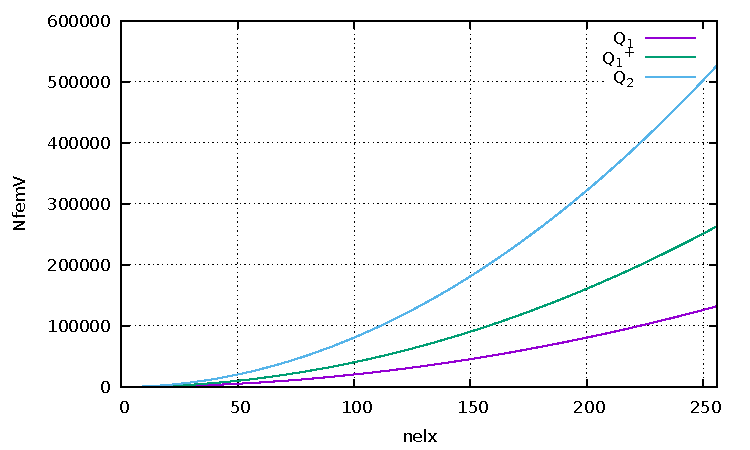
\includegraphics[width=8cm]{images/basis_q1p/NfemV_2D.pdf}
\end{center}




\Literature: 
\begin{itemize}
\item Mons \& Roge (1992) \cite{moro92}, 
\item Li \etal (2009) \cite{lihc09}, 
\item Knobloch \& Tobiska (2000) \cite{knto00}, 
\item Franca \etal (1993) \cite{frha93}, 
\item Idelsohn \etal (1995) \cite{idsn95}.
\end{itemize}

